\documentclass{article}

\usepackage{arxiv}

\usepackage[utf8]{inputenc} % allow utf-8 input
\usepackage[T1]{fontenc}    % use 8-bit T1 fonts
\usepackage{hyperref}       % hyperlinks
\usepackage{url}            % simple URL typesetting
\usepackage{booktabs}       % professional-quality tables
\usepackage{amsfonts}       % blackboard math symbols
\usepackage{nicefrac}       % compact symbols for 1/2, etc.
\usepackage{microtype}      % microtypography
\usepackage{graphicx}
\usepackage{natbib}
\usepackage{doi}
\usepackage{lipsum}
\usepackage{amsmath}
\usepackage{nicematrix}
\usepackage{cleveref}
\usepackage{svg}
\usepackage{listings}
\usepackage{pgfplots}
\usepackage{listings}

\usepackage{algpseudocode}
\usepackage{algorithm}

\usepackage{array}
\usepackage{booktabs}
\usepackage{siunitx}

\hypersetup{
    colorlinks=true,
    linkcolor=blue,
    filecolor=magenta,
    urlcolor=blue,
    pdftitle={Overleaf Example},
    pdfpagemode=FullScreen,
    }

\renewcommand{\algorithmicrequire}{\textbf{Input:}}
\renewcommand{\algorithmicensure}{\textbf{Initialize:}}

\lstset{
  basicstyle=\footnotesize, frame=tb,
  xleftmargin=.2\textwidth, xrightmargin=.2\textwidth
}

\NiceMatrixOptions{cell-space-top-limit=5pt,cell-space-bottom-limit=5pt,columns-width=20pt}

\Crefname{lstlisting}{listing}{listings}
\Crefname{lstlisting}{Listing}{Listings}


% Listing options
\definecolor{codegreen}{rgb}{0,0.6,0}
\definecolor{codegray}{rgb}{0.5,0.5,0.5}
\definecolor{codepurple}{rgb}{0.58,0,0.82}
\definecolor{backcolour}{rgb}{0.95,0.95,0.92}

\lstdefinestyle{python_style}{
    backgroundcolor=\color{backcolour},
    commentstyle=\color{codegreen},
    keywordstyle=\color{magenta},
    numberstyle=\tiny\color{codegray},
    stringstyle=\color{codepurple},
    basicstyle=\ttfamily\footnotesize,
    breakatwhitespace=false,
    breaklines=true,
    captionpos=b,
    keepspaces=true,
    numbers=left,
    numbersep=5pt,
    showspaces=false,
    showstringspaces=false,
    showtabs=false,
    tabsize=2
}
\lstset{style=python_style}
\NewDocumentCommand{\codeword}{v}{%
\texttt{\textcolor{blue}{#1}}%
}

\def\R{\mathbb{R}}


\title{Detecting AI-generated Python code via Machine Learning}

\date{}

\author{
  \hspace{1mm}Dmitry Beresnev\\
	AIDS-MS1, Innopolis University\\
	\texttt{d.beresnev@innopolis.university}\\
	\And{}
  \hspace{1mm}Vsevolod Klyushev\\
	AIDS-MS1, Innopolis University\\
	\texttt{v.klyushev@innopolis.university}	\And{}
  \hspace{1mm}Nikita Yaneev\\
	AIDS-MS1, Innopolis University\\
	\texttt{n.yaneev@innopolis.university}
}

\renewcommand{\undertitle}{Project report for AML course S25 Innopolis University}
\renewcommand{\headeright}{}

\pgfplotsset{compat=1.18}
\begin{document}
\maketitle

\section{Motivation}
Rapid advancement of artificial intelligence led to the widespread use of large language models in code generation, particularly in programming competitions. Although AI-generated code could help participants, it also raised concerns about fairness and originality in contests where human problem solving skills were evaluated. Detecting AI-generated code had to become an important task in ensuring the integrity of programming competitions.

Traditional methods of plagiarism detection were often insufficient for identifying AI-generated code, as LLMs could produce highly varied and syntactically correct solutions that differed from human-written code in subtle but detectable ways. Machine learning (ML) approaches offered a promising solution by analyzing patterns in code structure, style, and other latent features that distinguished machine-generated code from human-written code.

In this project, we explored different ML approaches to detect AI-generated Python code, because this was the most popular programming language. We compared two main strategies:


\begin{itemize}
  \item Pre-trained LLM-based detection --- leveraging a powerful but computationally heavy model to classify code based on deep semantic features
  \item Tree-based models --- utilizing lightweight decision trees or ensemble methods for faster inference and light weight, which is crucial in time-sensitive evaluation scenarios.
\end{itemize}

Our goal is to evaluate the trade-offs between accuracy and computational efficiency, ensuring that the solution is both reliable and practical for real-world programming competitions conducted on Accept~\cite{Beresnev}. Using these approaches, our aim is to develop a robust detection system that can help maintain fairness in coding contests while optimizing performance for large-scale use.

\section{Related work}

The detection of AI-generated code has gained significant attention with the recent rise of large language models (LLMs) like ChatGPT, Gemini, and GitHub Copilot. Previous studies have explored the detection of machine-generated text using stylometric and statistical techniques, often focusing on natural language (e.g.~\cite{Su2020}). Suh et al.\ proposed GPTSniffer, a fine-tuned CodeBERT model for Java code detection, but its ability to generalize to other languages such as Python remained limited~\cite{Suh24}. Additional work by Choi et al.\ investigated the attribution of authorship of source code through LLMs~\cite{Choi2025}. However, most of these studies have focused on general-purpose detection without specialization for Python or the nuances of specific model requirements. Our work extends this line of research by developing a targeted machine learning pipeline to identify generated Python code, considering the constraints on time consumption.

\section{Data generation}

First of all, the dataset of both human-written and AI-generated codes should be created. The final dataset include 12427 labeled code snippets.

\subsection{Human-written entities}

As human-written code snippets, anonymized Python solutions of Accept~\cite{Beresnev} platform users are used. Only valid solutions were used: for example, codes that resulted in a compilation error were omitted. In total, 5951 human-written solutions were included into dataset.

\subsection{AI-generated entities}

To generate AI-plagiarized code snippets, we decided to use the following LLM models:
\begin{itemize}
  \item \href{https://huggingface.co/DavidAU/L3.1-Evil-Reasoning-Dark-Planet-Hermes-R1-Uncensored-8B?not-for-all-audiences=true}{Evil}
  \item \href{https://huggingface.co/meta-llama/Llama-3.2-3B}{Llama-3.2-3b}
  \item \href{https://www.blackbox.ai/}{BLACKBOX.AI}
  \item \href{https://chat.deepseek.com/}{DeepSeek}
\end{itemize}

The tasks from Accept~\cite{Beresnev} (solutions of which resulted in human-written codes) were added to the following prompt and then passed to the LLM:

\medskip
\fbox{
  \parbox{0.9\linewidth}{
    \textit{Write a Python solution for the following task.
      The code should look like it was written by an intermediate student: practical but not overly optimized or perfect. Follow these guidelines:}

    \textit{1. Use not overly long names (e.g., res instead of result or final\_output\_value)}

    \textit{2. Do not include comments or explanations}

    \textit{3. Avoid using functions, prefer straightforward logic}

    \textit{4. Apply small stylistic deviations, like mixing single/double quotes, occasional redundant logic, inconsistent spacing, etc}

    \textit{5. No error handling}

    \textit{6. Do not print to output anything except answer to the problem without any annotations}

    \textit{Finally, return just pure python code}
  }
}
\medskip

Therefore, in total there are 6477 AI-generated code snippets.

\section{LLM approach}

We decided to check several LLM models to solve our problem - DeBERTaV3 and CodeBERT. To use them, we added a linear layer with 1 output and sigmoid activation function to predict the probability of text to be AI generated. We used Adam optimizer with learning rate 2e-5 and trained them for all models within 2 epochs achieving decent performance.

\subsection{DeBERTaV3}

DeBERTa~\cite{He2023} improves the BERT and RoBERTa models using disentangled attention and improved mask decoder. With those two improvements, DeBERTa outperforms RoBERTa in most natural language understanding (NLU) tasks.

\subsection{CodeBERT}

CodeBERT~\cite{Feng2020} --- bimodal pre-trained model for programming language (PL) and natural language (NL). CodeBERT learns general-purpose representations that support downstream NL-PL applications such as natural language code search, code documentation generation, etc.

\section{AST approach}
An Abstract Syntax Tree (AST) is a finite labeled oriented tree in which the inner vertices are mapped to programming language operators and the leaves to their corresponding operands.

To distinguish between human-written and AI-generated Python code, we employ an abstract syntax tree (AST)-based representation that captures the structural and syntactic patterns of the code. Unlike raw text-based or token-based methods, ASTs provide a more robust and hierarchical representation of code, making them suitable for detecting subtle differences in coding styles between humans and AI models.

The first step in our approach is to convert the Python source code into its AST representation. This is done using \href{https://tree-sitter.github.io/tree-sitter/}{Tree-setter} library, which parses the code into a tree structure where:

\begin{itemize}
  \item Nodes represent syntactic elements: functions, loops, conditionals, etc.
  \item Edges define the relationships between these elements
\end{itemize}

For example, for the code in \Cref{lst:code_ast}, Abstract Syntax Tree is depicted in \Cref{fig:ex_ast}.

\begin{lstlisting}[language=Python,frame=single,caption=Python code snippet,label=lst:code_ast]
a = 10
b = 5
if a < b:
    c = a
\end{lstlisting}

\begin{figure}[H]
  \centering
  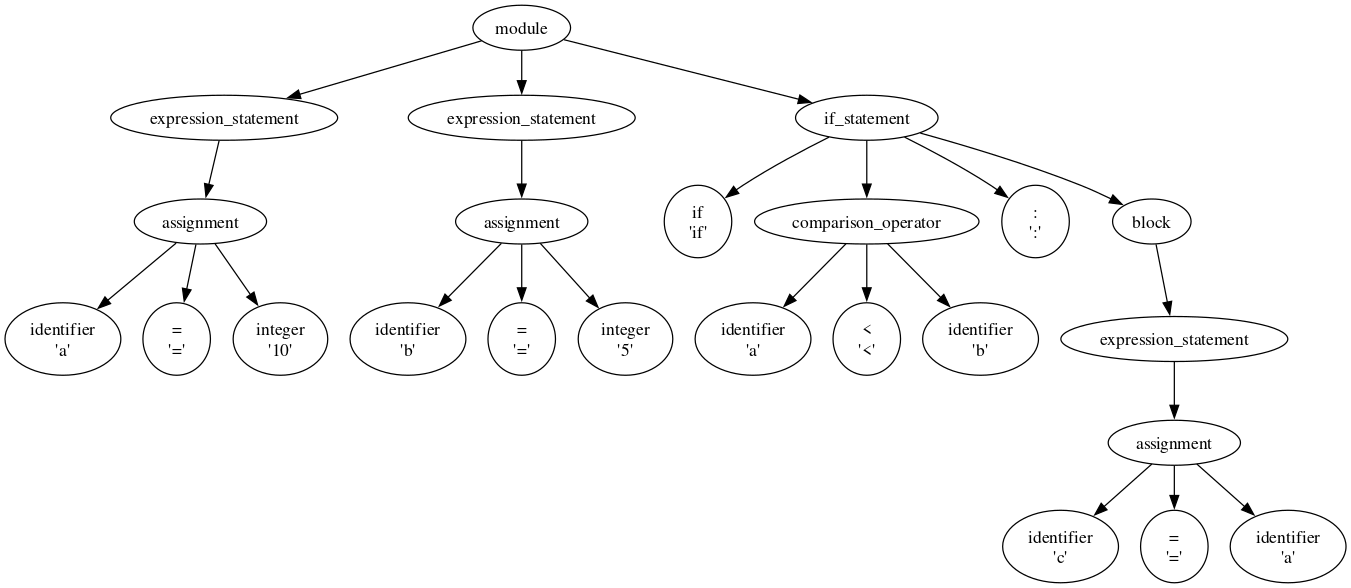
\includegraphics[width=0.95\textwidth]{./pictures/ast_output.png}
  \caption{Example of AST}\label{fig:ex_ast}
\end{figure}

\subsection{Decision Tree and Random Forest}
To complement the computationally expensive LLM-based approach, we explored lightweight yet effective tree-based models --- Decision Trees and Random Forest --- trained on Abstract Syntax Tree (AST) features. These models provide a strong balance between performance and efficiency, making them particularly suitable for deployment in programming competitions where fast inference is critical.

The key advantage of tree-based models lies in their interpretability and speed. Unlike deep learning models, which require significant computational resources, Decision Trees and Random Forests process structured data efficiently, making them ideal for real-time detection systems. By encoding Python code into AST-based features, we enable these models to learn distinguishing patterns between human-written and AI-generated code.

However, a notable limitation of tree-based approaches is their reliance on static feature representations. As AI code generation models evolve—with new architectures, fine-tuning techniques, and prompt engineering strategies—the statistical patterns in generated code may change over time. This means that tree-based models, while highly performance in deployment, require periodic retraining on updated datasets to maintain detection accuracy. Without regular updates, their effectiveness may degrade as newer AI models produce code that diverges from previously learned patterns.

Despite this constraint, Decision Trees and Random Forests remain a practical choice for scenarios where low-latency inference is essential. Their ability to deliver high accuracy with minimal computational overhead makes them a compelling alternative to heavy-weight LLM-based detectors, especially in resource-constrained environments such as automated classification systems or programming competitions. For long-term robustness, a hybrid approach --- combining periodic retraining of tree-based models with occasional LLM-based verification --- could offer the best trade-off between speed and adaptability.

\subsection{Multi-Layer Perceptron}
To complement tree-based methods like Decision Trees and Random Forests, we also explored a Multi-Layer Perceptron (MLP) approach for detecting AI-generated Python code. The MLP model consists of four linear layers with LeakyReLU activation functions and dropout layers for regularization. The input to the network consists of embeddings derived from the Abstract Syntax Tree (AST) representation of the code, and the output is a probability score indicating whether the code was AI-generated. This neural network approach provides a more sophisticated, non-linear alternative capable of capturing complex patterns in the data while maintaining robustness through dropout regularization. The MLP serves as an additional method in our comparative analysis of different techniques for AI-generated code detection.

\section{Evaluation and comparison}

\subsection{Comparison of models}

The results of the proposed approaches are shown on \Cref{tab:model_comparison}. As you can notice, the CodeBERT-base model demonstrated the best performance in terms of all metrics: F1 score, Roc/Auc, Precision, Recall and Accuracy. However, at the same time it is the second biggest and slowest model. The AST-based Random Forest is the fastest, though its metrics are still descent.
\begin{table}[ht!]
  \small
  \centering
  \caption{Comparison of models}\label{tab:model_comparison}
  \begin{tabular}{llllllll}
    \toprule
    Model                      & {F1}           & {ROC/AUC}      & {Precision}    & {Recall}       & {Accuracy}     & {Time (s)}     & {Memory (MB)} \\
    \midrule
    \textbf{DeBERTa-v3-xsmall} & 0.899          & 0.890          & 0.870          & 0.930          & 0.891          & 0.07           & 269           \\
    \textbf{DeBERTa-v3-base}   & 0.903          & 0.899          & 0.902          & 0.904          & 0.899          & 0.13           & 701           \\
    \textbf{CodeBERT-base}     & \textbf{0.959} & \textbf{0.959} & \textbf{0.978} & \textbf{0.941} & \textbf{0.958} & 0.07           & 475           \\
    \textbf{Random Forest AST} & 0.841          & 0.835          & 0.834          & 0.847          & 0.835          & \textbf{0.002} & 5.8           \\
    \textbf{MLP AST}           & 0.787          & 0.785          & 0.809          & 0.767          & 0.784          & 0.004          & \textbf{0.06} \\
    \bottomrule
  \end{tabular}
\end{table}

\subsection{Interpretability}

In order to interpret decisions of our models, we decided to add Local Interpretable Model-agnostic Explanations (LIME)~\cite{Ribeiro16} to our pipeline.

For example, for the code in \Cref{lst:code_lime}, the LIME explanations for AST Random Forest and CodeBERT models are shown in \Cref{fig:LIME_AST,fig:LIME_CodeBERT} respectively.

\begin{lstlisting}[language=Python,frame=single,caption=Python code snippet,label=lst:code_lime]
n = int(input())
a = sorted(map(int, input().split()))
b = sorted(map(int, input().split()))
s = 0
for i in range(n-1, -1,-1):
    s += abs(a[i]-b[i])
print(s)
\end{lstlisting}

\begin{figure}[H]
  \centering
  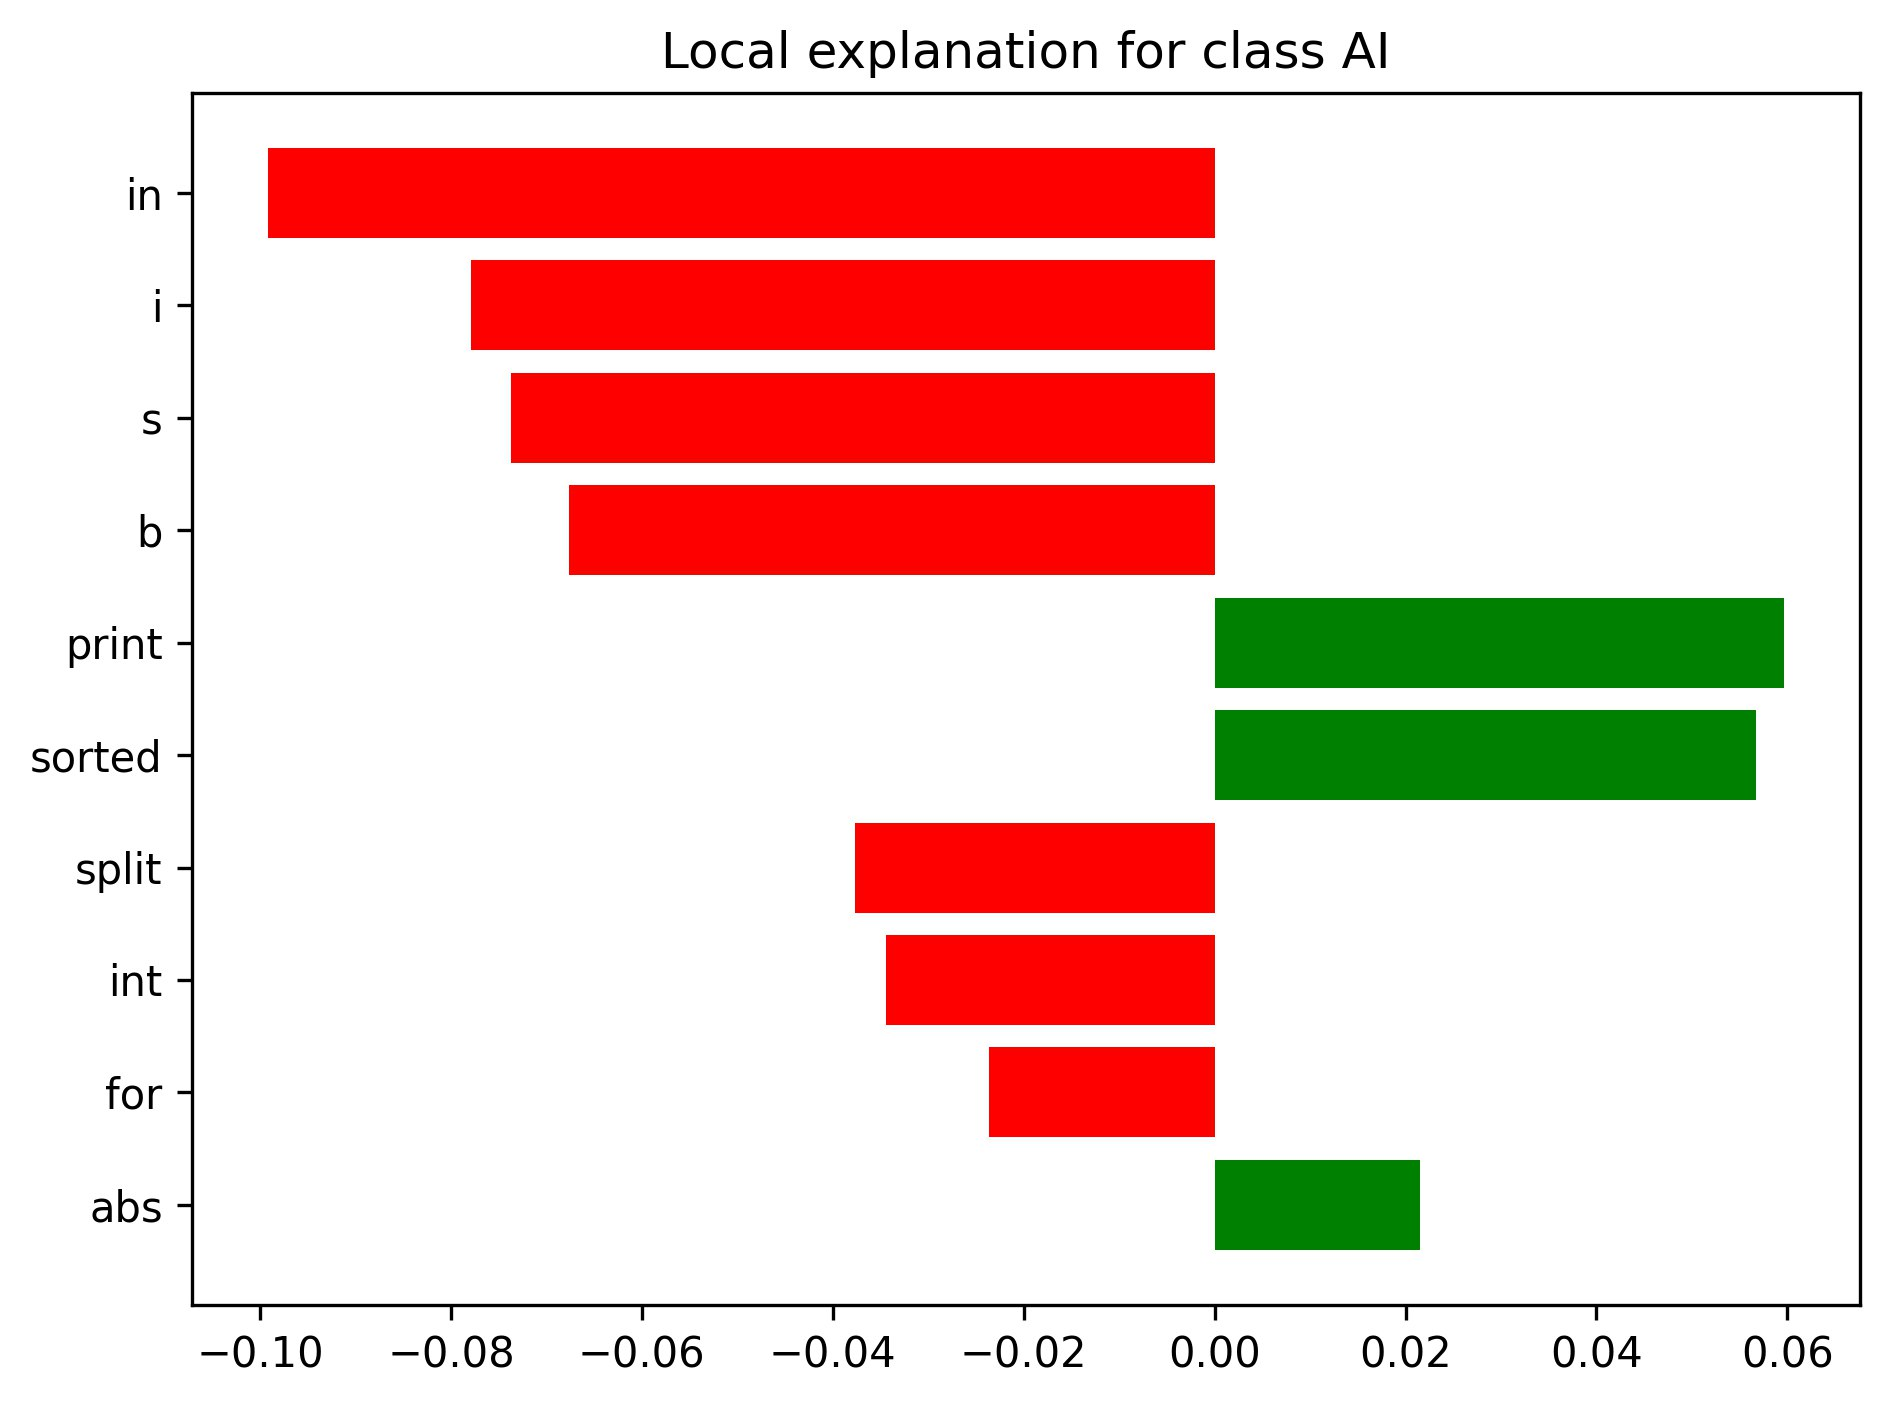
\includegraphics[width=0.5\textwidth]{./pictures/ast_lime.jpg}
  \caption{Lime explanation for AST RF}\label{fig:LIME_AST}
\end{figure}

\begin{figure}[H]
  \centering
  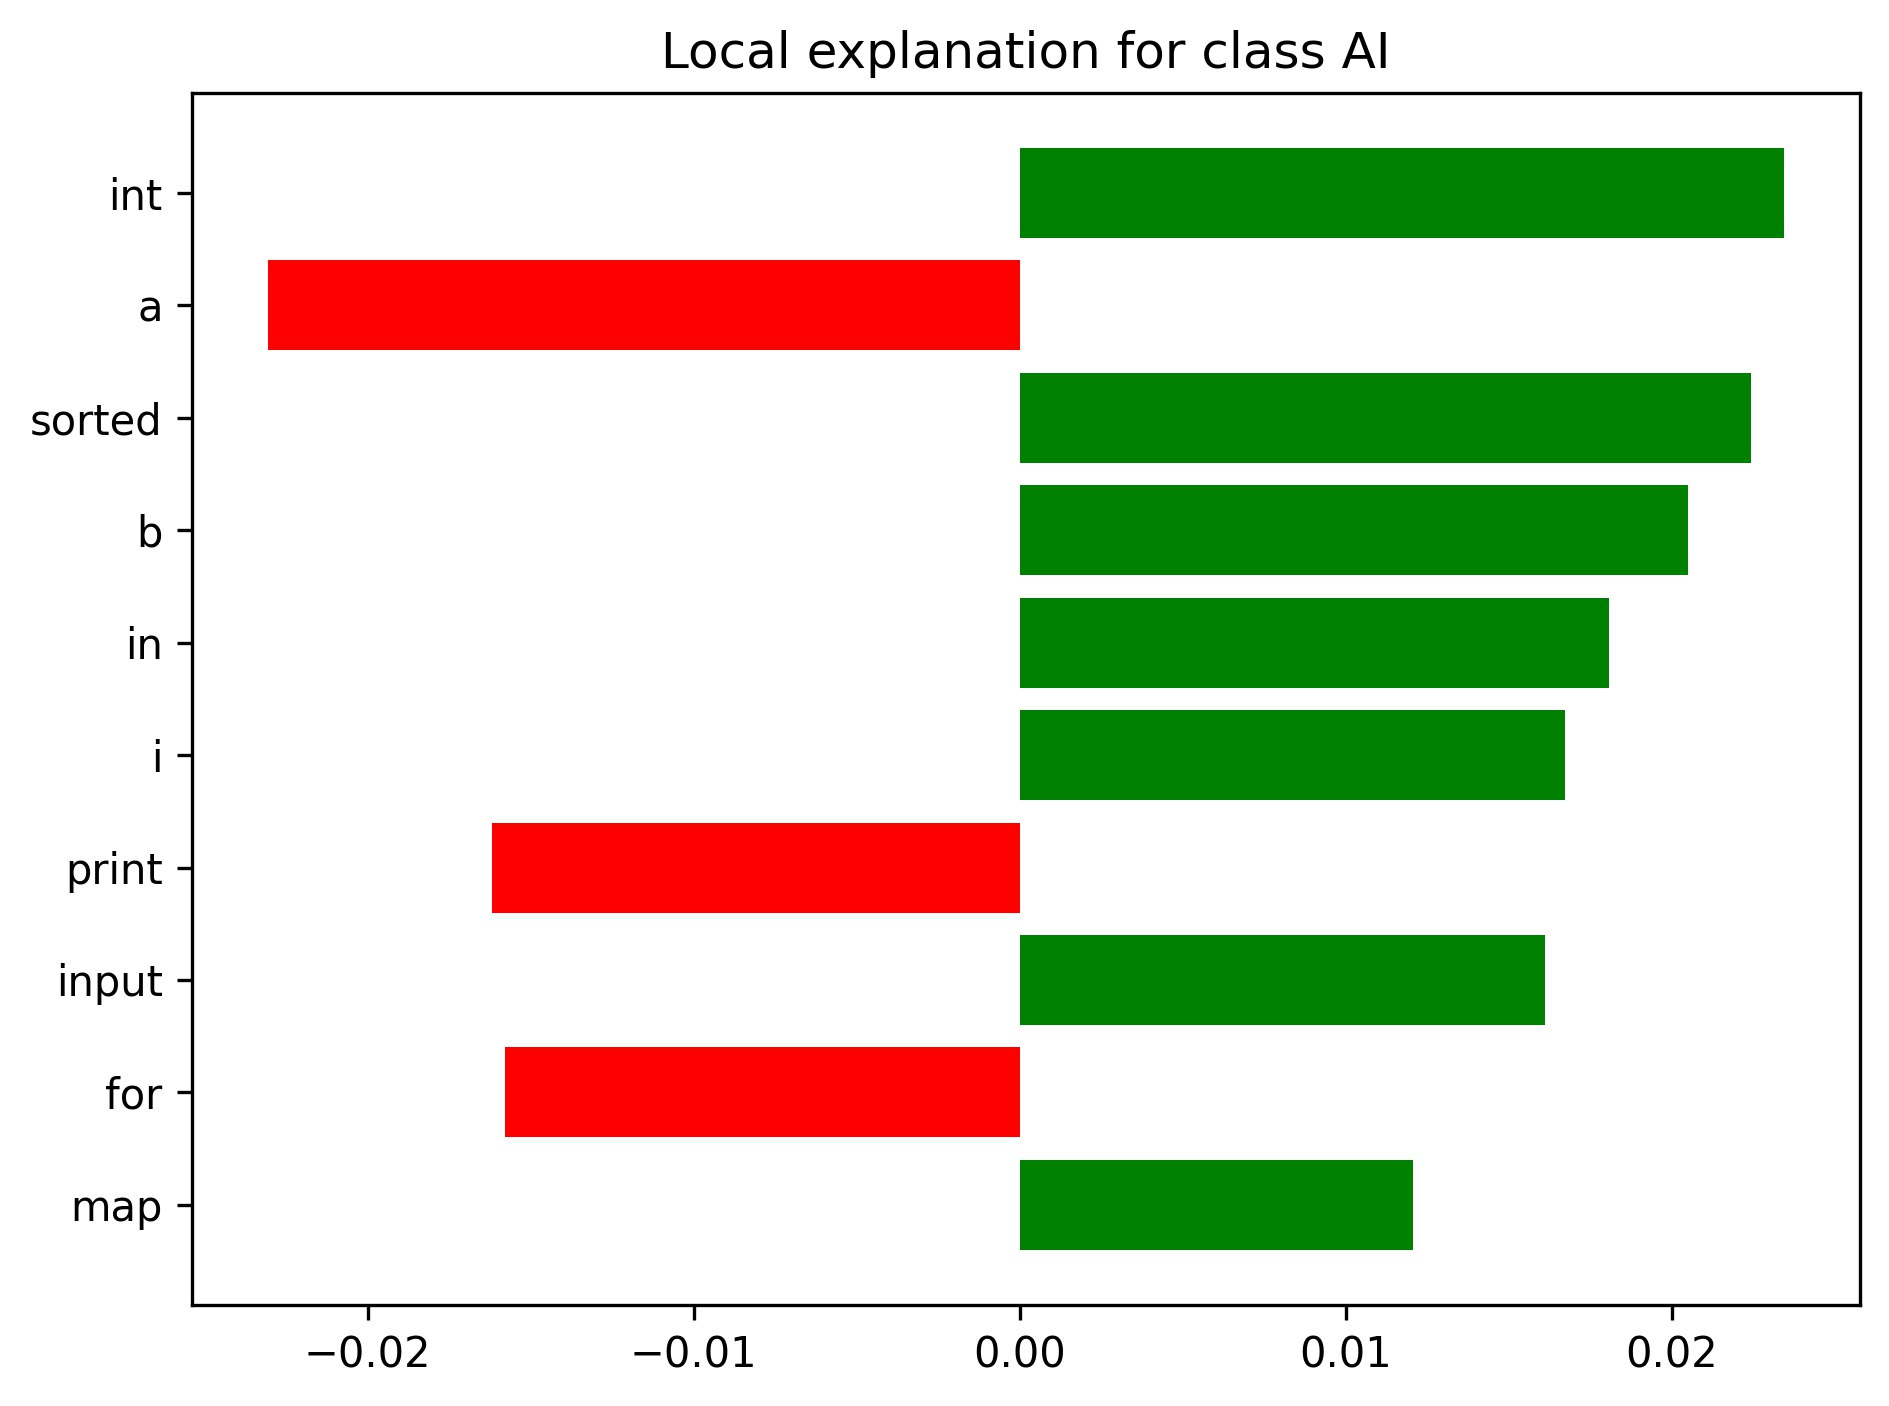
\includegraphics[width=0.5\textwidth]{./pictures/codebert_lime.jpg}
  \caption{Lime explanation for CodeBERT}\label{fig:LIME_CodeBERT}
\end{figure}

The explanation provided by LIME for both models might seem to be unsatisfactory due to applied time constraints to keep fast inference. Also, the principle of LIME work includes generating perturbations, which can result in strange and not existing code embeddings, hence the explanations can be possibly limited for interpretation.

\section{Deployment}

We decided to deploy our CodeBERT and AST Random Forest models via a Telegram bot with help of \texttt{aiogram} library. We choose such models, since they show best performance for each approach. You can access bot \href{https://t.me/ui_ai_detector_bot}{here}\footnote{If the bot is down, write \href{https://t.me/Kiaver}{Vsevolod Klyushev}}.

\section{GitHub}

You can check GitHub of this project \href{https://github.com/dsomni/ml-s25}{here}.

\section{Results and Discussion}

We successfully implemented models for AI code detection, which might be used inside Accept~\cite{Beresnev} system. Both the AST-based and LLM-based approaches showed excellent performance. While CodeBERT wins in terms of metrics, AST-based Random Forest Classifier is much faster and less memory consuming, so it can be considered as the best solution in terms of proposed constraints: throughput and memory limitations. Also, the LIME was used to explain the decision of selected models. Finally, the Telegram bot was deployed for demonstration purposes.

\bibliographystyle{plain}
\bibliography{references}


\end{document}